\documentclass[tikz, border=10pt]{standalone}
\usepackage{tikz}
\usetikzlibrary{patterns}

\begin{document}
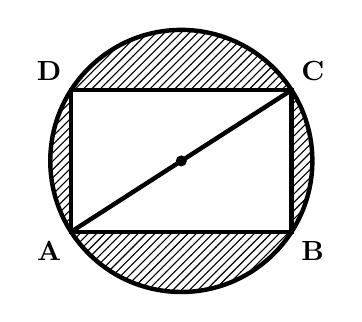
\begin{tikzpicture}

% Define half-width and half-height of rectangle
\def\w{1.4}
\def\h{0.9}

% Calculate radius (diagonal of rectangle / 2)
\pgfmathsetmacro{\r}{sqrt(\w*\w + \h*\h)}

% Center point
\coordinate (O) at (0,0);

% Rectangle corners (inscribed in circle)
\coordinate (A) at (-\w, -\h);
\coordinate (B) at (\w, -\h);
\coordinate (C) at (\w, \h);
\coordinate (D) at (-\w, \h);

% Draw hatched circle (pattern first)
\fill[pattern=north east lines, pattern color=black] (O) circle (\r);

% Fill rectangle with white to remove pattern inside
\fill[white] (A) -- (B) -- (C) -- (D) -- cycle;

% Draw circle outline
\draw[ultra thick] (O) circle (\r);

% Draw rectangle
\draw[ultra thick] (A) -- (B) -- (C) -- (D) -- cycle;

% Draw diagonal from A to C
\draw[ultra thick] (A) -- (C);

% Draw center point
\fill (O) circle (2pt);

% Labels
\node[below left] at (A) {\textbf{A}};
\node[below right] at (B) {\textbf{B}};
\node[above right] at (C) {\textbf{C}};
\node[above left] at (D) {\textbf{D}};

\end{tikzpicture}
\end{document}